\section{Introduction}\label{sec:intro}
% Problem, importantness, and specific question
Reward is a fundamental brain function that shapes our behavior through reward-based learning, or reinforcement learning (RL). Positive rewards encourage us to eat food and find mating partners, while negative rewards, such as pain and fatigue, help us protect ourselves. However, regardless of its importance to animal lives, the evolutionary process of such a reward system is underexplored. Reward signals should have evolved to help animals survive and reproduce offspring (e.g., by~\cite{schultzNeuronalRewardDecision2015}), but what kind of environmental conditions have influenced the evolution of varieties of rewards remains unclear.

\begin{figure}[t]
  \centering{}
  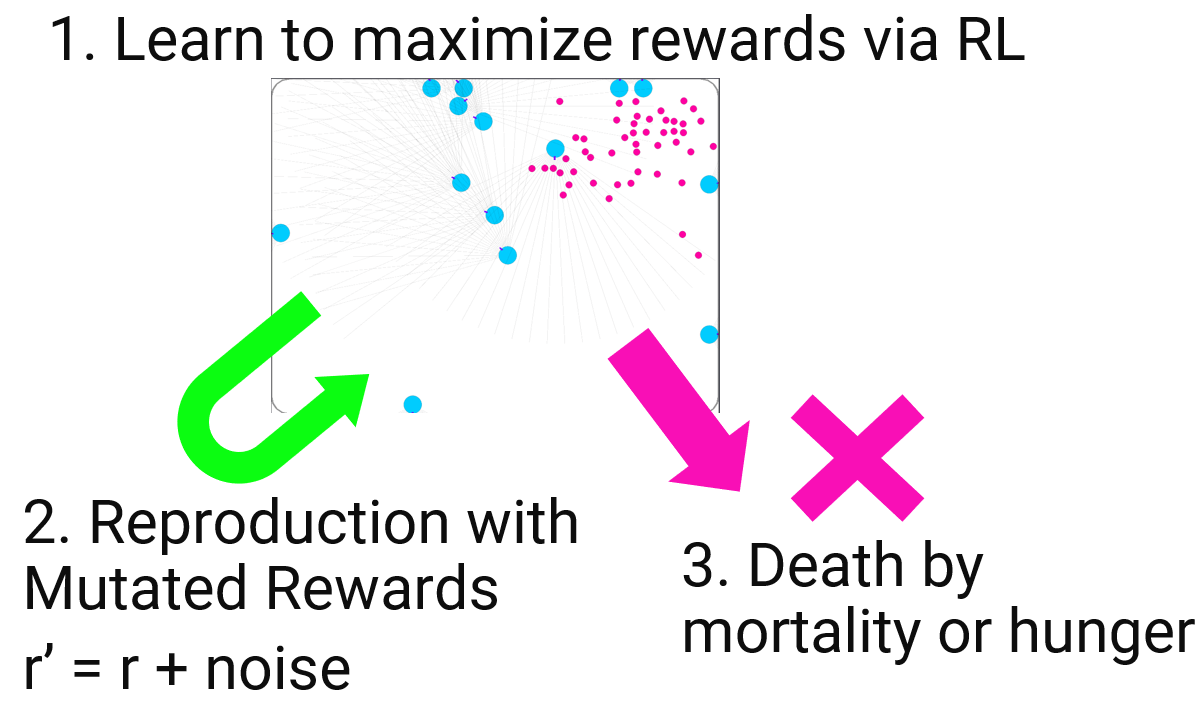
\includegraphics[width=7cm]{emevo-scheme2-min.png}
  \caption{
    A schematic figure on our evolutionary framework.
    Aagens learn to maximize their reward functions inherited from their parents.
    They reproduce children with mutated reward functions and die from aging or hunger.
  }\label{figure:scheme}
\end{figure}


% What we do
While biological studies in evolution are important, the difficulty of observing reward evolution in real animals motivates us to use artificial evolutionary simulation. Hence, we conduct an evolutionary simulation of RL agents to examine how different environmental conditions lead to different rewards. Each agent inherits a reward function from its parent and learns to get more rewards by RL during its lifetime. Contrary to previous studies on the evolution of learning \citep{hintonHowLearningCan1987,singhWhereRewardsCome2009} with centralized selection strategies, we design a distributed evolutionary model inspired by embodied evolution (EE) framework \citep{watsonEmbodiedEvolutionDistributing2002,bredecheEmbodiedEvolutionCollective2018}. In our model, birth and death for agents are evaluated independently based on their age and internal energy level, allowing the population change. With this approach, we expect rewards contributing to population growth to be selected. We show a schematic figure on our evolutionary framework in \Cref{figure:scheme}.

% Foraging environment
% Simulation
We implement our distributed evolution framework in a simple virtual environment where agents need to hunt foods to live longer and produce children based on 2D physics simulation. In this environment, we let agents evolve simple reward functions that map food intake and the magnitude of motor output to a scalar, which we expect to correspond to food pleasure and fatigue. Our results show that biologically reasonable reward functions with positive food rewards and negative action rewards evolve from randomly initialized ones. We then find that metabolic balance, food density, and food relocation influence rewards for taking motor action, while food rewards are consistently positive. Furthermore, we examine the evolution of rewards for poor and poisonous rewards, showing the instability of less important foods and the stability of normal foods are consistently positive. Overall, our results demonstrate the usefulness of our simulation environment and distributed evolution model for further studies. We then conclude the paper by discussing possible improvements and future works.

\section{Preliminaries and Related Works}\label{sec:related}
We follow the standard computational RL framework \citep{suttonReinforcementLearningIntroduction2018} based on the Markov decision process (MDP). MDP $\M{}$ consists of a tuple $(\X{}, \A{}, p, r, \gamma)$, where $\X{}$ is reward function, and $\gamma \in [0, 1]$ is the discount factor. A standard objective in MDP is the discounted cumulative return $G \defequal{} \sum_{t=0}^{\infty}\gamma^t R_{t}$, where $R_t$ is the reward received at time $t$. An RL agent has policy $\pi: \X \times \A \rightarrow [0, 1]$ and seeks to find the the optimal policy $\pi^{*}$ that maximizes $\E \left[G|\pi\right]$. The state-value function $V^\pi(s) \defequal \sum_{a \in \A} \pi(a|s) \left( r(s, a) + \gamma \sum_{s' \in \X} P(s'|s, a) V^\pi(s') \right)$ is often used in RL algorithms. Observation $o \in \Omega~(\Omega \subseteq \X)$ refers to a part of the state that an agent can observe.

Our reward model is inspired by the neuroscience of reward system \citep{schultzNeuronalRewardDecision2015, berridgePleasureSystemsBrain2015}. Notably, \citet{berridgeDissectingComponentsReward2009} argue that the brain reward system consists of three independent components: liking, wanting, and learning. In analogy with computational RL, liking corresponds to reward function, wanting corresponds to learned policy, and learning corresponds to learning state value $V$.

While there were previous attempts to evolve rewards in a single-agent setting \citep{singhWhereRewardsCome2009,niekumEvolutionRewardFunctions2011,zhengWhatCanLearned2020},
%While evolutionary robotics studies \citep{nolfiEvolutionaryRoboticsBiology2004} often employ a centralized selection scheme similar to genetic algorithm \citep{mitchellIntroductionGeneticAlgorithms1998},
%where highly evaluated elites are selected as parents. On the contrary,
we employ a distributed embodied evolution (EE) framework \citep{watsonEmbodiedEvolutionDistributing2002,bredecheEmbodiedEvolutionCollective2018} with many agents and population dynamics.
While the mainstream of evolutionary robotics studies \citep{nolfiEvolutionaryRoboticsBiology2004} employs a centralized elite selection, agents evolve locally following birth and death rules in EE. This method has the advantage that the evaluation of genetic traits depends on population dynamics and is more natural.

Our work is inspired by the series of studies \citep{elfwingBiologicallyInspiredEmbodied2005,elfwingDarwinianEmbodiedEvolution2011,elfwingEmergencePolymorphicMating2014}, which tried to evolve parameters related to RL through EE framework. Notably, \citet{elfwingDarwinianEmbodiedEvolution2011} evolved supplementary sharing rewards and parameters of RL agents.
Inspired by these works, we attempt to evolve the entire reward functions in our experiments.

\section{Simulation Model and Environment}\label{sec:method}

\begin{figure}[t]
  \centering{}
  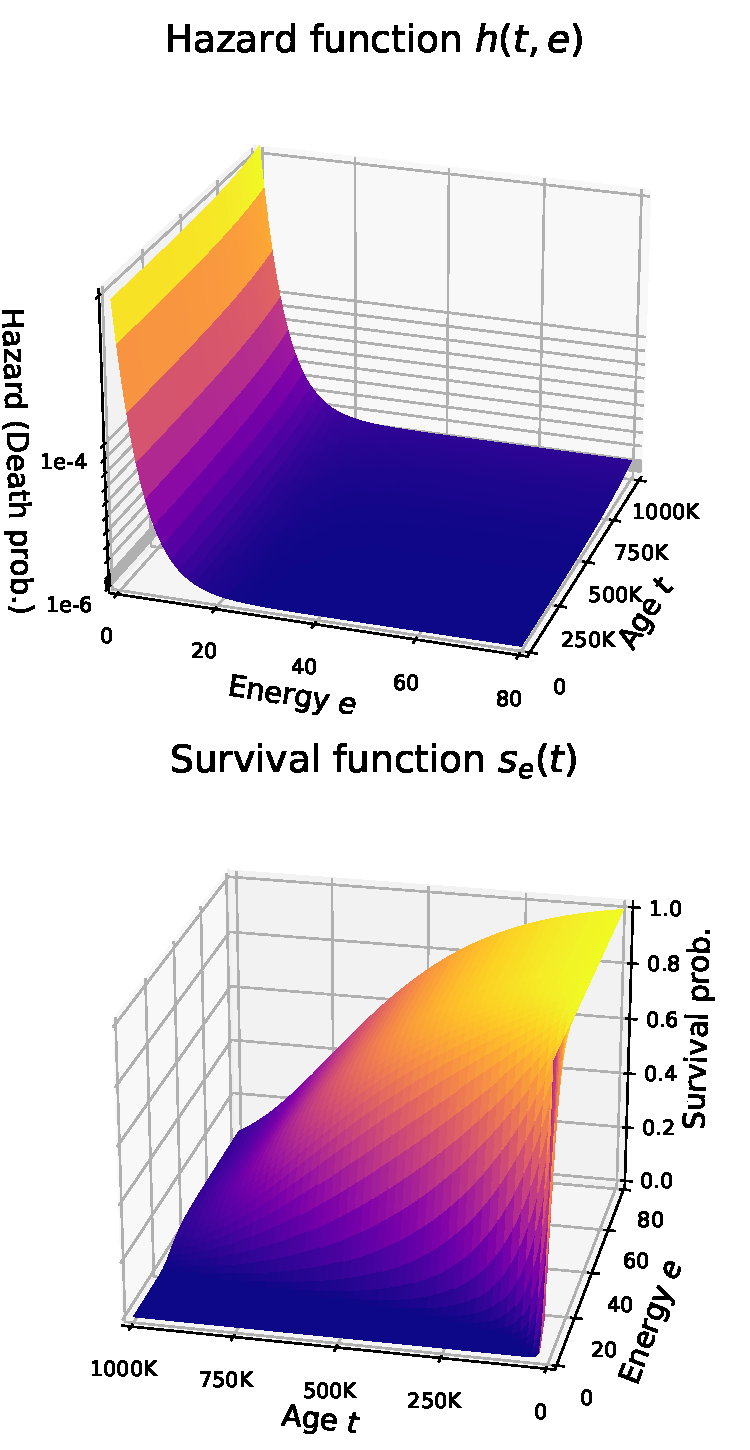
\includegraphics[width=6cm]{hazard_and_survival.pdf}
  \caption{
    \textbf{Upper:} Hazard function $h(t)$ used in our experiments.
    \textbf{Lower:} Survival function $S(t)$ corresponding to the hazard function above.
  }\label{figure:hs}
\end{figure}

\paragraph{Energy-based death and birth model}
We employ an energy-based metabolic model similar to \citet{hamonEcoevolutionaryDynamicsNonepisodic2023}. Each agent maintains their energy level $e$, which increases by eating food and decreases by the basal metabolism and taking a motor action.
The death probability of the agent with energy level $e$ and age $t$ is modeled by the hazard function:
\begin{align}
  h(t, e) = \frac{\kappa_{h}}{1 + \alpha_{e}\exp(\beta_{he}e)} + \alpha_{t} \exp(\beta_{ht} t).
  \label{eq:h}
\end{align}
The first term in \Cref{eq:h} increases as energy levels decrease following a sigmoidal curve where $\kappa_{h}$ is the scale, $\beta_{he}$ is the slope, and $\alpha_{e}$ defines the shape when $e=0$. The latter term increases exponentially as the agent ages with the cale $\alpha_{t}$ and the slope $\beta_{ht}$, called Gompertz hazard model \citep{gompertzXXIVNatureFunction1825,kirkwoodDecipheringDeathCommentary2015}.
We show the shape of $h$ with parameters used in our experiments in the upper panel in \Cref{figure:hs}. The lower panel in \Cref{figure:hs} shows the survival function $s_{e}(t) = \exp (-\int_{0}^{t}(h(t, e)) dt)$ corresponding to $h$, which is the probability for an agent to survive to the age $t$ under the assumption that it keeps the same energy level $e$. We can see that the survival probability more sharply decays with aging when the energy level is low.

\begin{figure}[t]
  \centering{}
  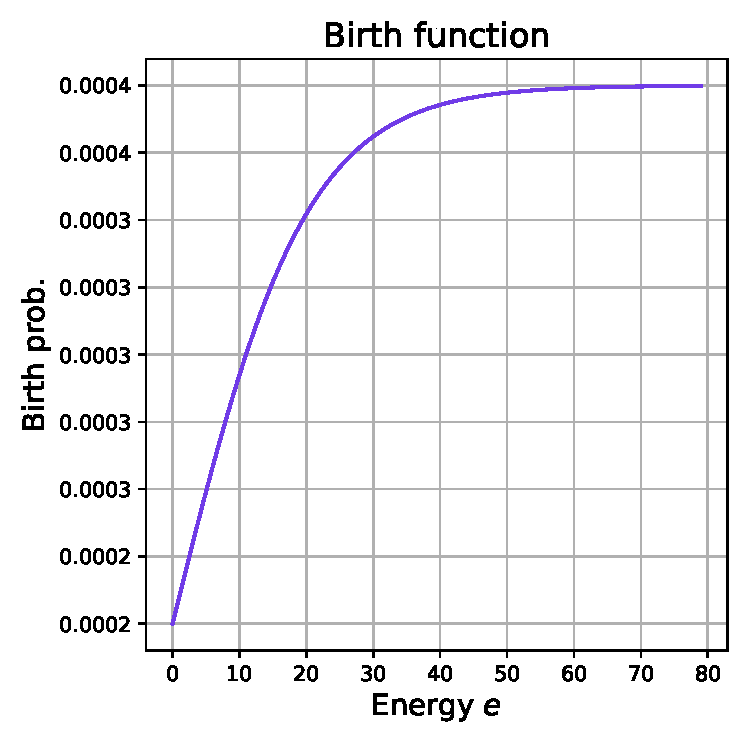
\includegraphics[width=6cm]{birth.pdf}
  \caption{Birth function $b(e)$ used in our experiments.}\label{figure:birth}
\end{figure}

\begin{table}[t]
  \begin{subtable}[h]{0.45\columnwidth}
    \centering
    \begin{tabular}{cc}
      \toprule
      Parameter & Value \\
      \midrule
      $\kappa_{h}$ & 0.01 \\
      $\alpha_{e}$ & 0.02 \\
      $\beta_{he}$ & 0.2 \\
      $\alpha_{ht}$ & \num{2e-7} \\
      $\beta_{t}$ & \num{4e-6} \\
      \bottomrule
    \end{tabular}
  \end{subtable}
  \begin{subtable}[h]{0.45\columnwidth}
    \centering
    \begin{tabular}{cc}
      \toprule
      Parameter & Value \\
      \midrule
      $\kappa_{b}$ & \num{4e-4} \\
      $\beta_{b}$ & 0.1 \\
      \bottomrule
    \end{tabular}
  \end{subtable}
  \caption{Parameters of $h$ (left) and $b$ (right) used in our experiments.}\label{table:hb}
\end{table}

For simplicity, we employ an asexual reproduction model with the birth function, the probability for an agent with energy level $e$ to produce a child in a time step:
\begin{align}
 b(e) &= \frac{\kappa_{b}}{1 + \exp(\beta_{b}e)}.
 \label{eq:b}
\end{align}
The birth rate $b(e)$ increases with $e$ following a sigmoidal curve where $\kappa_{b}$ is the scale and $\beta_{b}$ is the slope.
\Cref{figure:birth} shows the shape of $b$ for the parameters used in our experiments. We show all paramters of $h$ and $b$ in \Cref{table:hb}. With this choice of parameters, we expect the maximum lifetime of an agent to be around \num{1e6} steps.

\paragraph{Environment}

\begin{figure}[t]
  \centering
  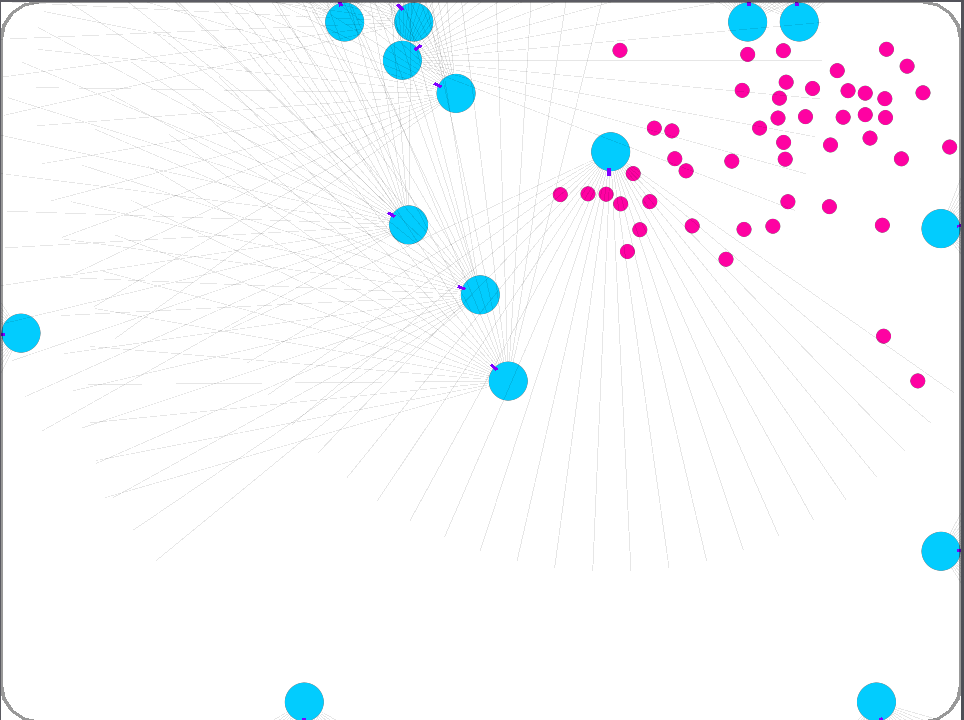
\includegraphics[width=6cm]{emevo-ss.png}
  \caption{
    Simulation environment used in our experiments.
    Blue circles are agents, red circles are foods, and outer gray lines are walls.
    Thin gray lines around agents indicate distance sensors.
  }\label{figure:env}
\end{figure}

\begin{figure}[t]
  \begin{subfigure}[t]{4.5cm}
    \centering
    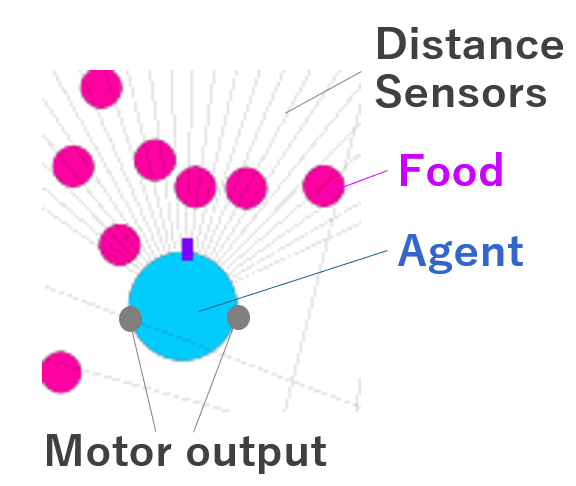
\includegraphics[width=4.5cm]{emevo-annot4-min.png}
  \end{subfigure}
  \begin{subfigure}[t]{3.5cm}
    \centering
    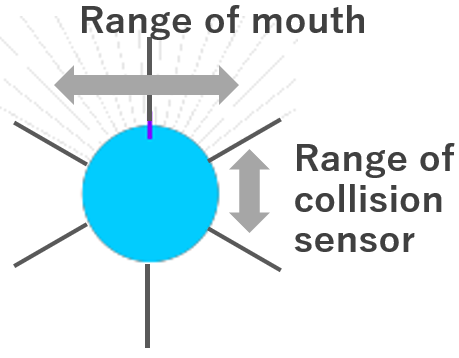
\includegraphics[width=3.5cm]{emevo-mouth.png}
  \end{subfigure}
  \caption{
    Description of the environment.
    The left figure shows an agent, foods, distance sensors, and the positions of motor outputs.
    The right figure shows the ranges of an agent's mouth and each collision sensor.
  }\label{figure:env-discr}
\end{figure}

We designed a continuous 2D environment shown in \Cref{figure:env}. Blue circles indicate agents, red circles indicate foods, and the outer gray lines are impassable walls. The environment is implemented by a 2D rigid-body physics simulation. Agents can move by producing driving forces on the left and right sides of the body, as shown in \Cref{figure:env-discr}. An agent has multiple range sensors in its front that can sense the type and distance to the closest object within $120$ degree. Sensible objects include foods, other agents, and walls. In environments with poor or poisonous foods, agents can sense them separately from normal foods. They can also sense the collision with each object and the approximate location of the collision with a resolution of $60$ degree, as shown in \Cref{figure:env-discr}.

% This eat-driven emergence is not consistent with the growth model below. Better report the actual food-producing process rather than theoretical approximation.
The agent can eat food by touching it within $120$ degrees of the front as shown in the right figure in \Cref{figure:env-discr}. By eating one food, it gains energy $e_{\mathrm{food}}$. We use $e_{\mathrm{food}} = 1$ in our experiments. In experiments with less nutrient-poor or poisonous foods, they have different energy gain $e_{\mathrm{poor}} = 0.2$ and $e_{\mathrm{poison}} = -0.4$. After foods are eaten, they are regenerated in a random place. To regulate the rate of food regeneration, we maintain the internal food number $n_{t}$ at time $t$ which follows a logistic growth function: $n_{t + 1} = n_{t} + gn_{t}(1 - \frac{n_{t}}{n_{\mathrm{max}}}) - n_{t}^{\mathrm{eaten}}$, where $g$ is the growth rate, $n_{\mathrm{max}}$ is the capacity of food, and $n_{t}^{\mathrm{eaten}}$ is the number of eaten foods at time $t$. Food is regenerated when the integer part of $n^{t}$ is more than the actual number of foods in the environment. We use $n_{\mathrm{max}} = 50$ and $g = 0.01$ in our experimens.

The agent consumes energy via active and basic metabolism. At each step $t$, An agent $i$ losts energy $e_{\mathrm{act}} |a_{t}^{i}|$, where $|a_{t}^{i}|$ is the Euclid norm of the agent's motor output $a_{t}^{i}$ and $e_{\mathrm{act}}$ is a scaling coefficient. In addition, it also consumes energy $e_{\mathrm{basic}}$ at every step. In our experiments, we use $e_{\mathrm{act}} = \num{2e-5}$ and $e_{\mathrm{basic}} = 0.001$, leading to the consumption of $0.002 \sim 0.003$ energy by one step. It means that agents need to eat food at least once in $500$ or $1000$ steps to maintain their energy level.

When an agent makes a child, a new agent is placed in a random location sampled from a Gaussian distribution centered around its parent. Reproduction fails when all $10$ sampled locations are not available. The child inherits a proportion of the parent's energy $\eta e$, and the parent's energy level decreases to $(1-\eta)e$, where $\eta \in [0, 1]$ is the ratio of energy sharing. We used $\eta = 0.4$ in our experiments. The child also inherits its reward function from the parent with some mutation, as described later.

Since we need many agents for evolution, the multi-agent interaction can be a huge bottleneck in our simulation. To overcome this challenge, we implement our environment using JAX Python library \citep{jax2018github} so that the entire simulation loop is executed on GPU. Inspired by recent works on 3D rigid body physics simulation using JAX (e.g., \citet{brax2021github} and MuJoCo \citep{todorov2012mujoco} MJX\footnote{\url{https://mujoco.readthedocs.io/en/stable/mjx.html}}), we implement our 2D physics engine using JAX and build our environment on top of that, optimizing it for multi-agent setting. Our simulator implements projected Gauss-Seidel method with position correction \citep{catto2005iterative} that is pretty common in 2D game physics engines such as Box2D\footnote{\url{https://box2d.org}} and Chipmunk\footnote{\url{https://chipmunk-physics.net}}. We plan to release our simulation framework as open source after publication.

\paragraph{Reward Function with Evolving Weights}
We assume that the reward function is determined at birth with mutation and does not change during the agent's lifetime. We use food intake and the magnitude of the agent's action (motor output) as inputs to the reward function. We expect a positive food reward to evolve to acquire energy and a negative reward for action to evolve to save energy.
We model the reward of an agent $i$ at time $t$ by:
\begin{align}
  r^{i}_{t} = w_{\mathrm{food}}^{i}n_{t}^{i} + c_\mathrm{act} w_{\mathrm{act}}^{i}|a_{t}^{i}|\label{eq:rew}.
\end{align}
In \cref{eq:rew}, $n_{t}^{i}$ is the number of foods that the agent at that step, and $w_{\mathrm{food}}^{i}$ and $w_{\mathrm{act}}^{i}$ are evolvable reward parameters of an agent $i$. Because an agent gets the action reward at every step but doesn't get the food reward so often, we use a fixed parameter $c_\mathrm{act}$ to scale the reward. We use $c_\mathrm{act}=0.01$ in our experiments. In experiments with poor or poisonous foods, we use another evolvable reward parameter $w_{\mathrm{poor}}^{i}$ or $w_{\mathrm{poison}}^{i}$.

The newborn inherits reward parameters $w_{\mathrm{food}}$ and $w_{\mathrm{act}}$ from its parent with some mutation added. To allow large jumps, we sample mutation noise from the Cauchy distribution with the scale parameter $0.02$ independently for each reward weight. After added Cauchy noise, each parameter is clipped to the range $[-10, 10]$ to prevent too large jumps.

\begin{table}[t]
  \centering
  \caption{RL parameters}\label{tab:rl-param}
  \begin{tabular}{ll}
    \toprule
    Parameter & Value \\
    \midrule
    Discount factor ($\gamma$) & 0.999 \\
    Rollout steps ($N$) & 1024 \\
    Minibatch size & 256 \\
    Number of optimization epochs & 10 \\
    PPO Clipping parameter & 0.2 \\
    Entropy coeff. & 0.0 \\
    GAE parameter ($\gamma$) & 0.95 \\
    Adam learning rate & \num{3e-4} \\
    Adam $\epsilon$ & \num{1e-7} \\
    Size of hidden layer in MLP & 64 \\
    \bottomrule
  \end{tabular}
\end{table}

\paragraph{Reinforcement Learning}
We use Proximal Policy Optimization \citep{schulmanProximalPolicyOptimization2017} as an RL algorithm because of its fast computation time. In addition to the touch and collision sensor inputs in \Cref{figure:env-discr}, the agent takes its angle, velocity, and energy level as an observation. The action space is a continuous two-dimensional vector corresponding to the forces applied to the left and right sides of the body, clipped to $[-20, 80]$. Following the standard practice in the literature, we use a multi-layer perception (MLP) with hyperbolic tangent activation to represent the agent's policy, which is randomly initialized for each newborn. We show RL parameters used in our experiments in \Cref{tab:rl-param}.

% Add a line for reward acquisition; after observation or action?
\begin{algorithm}[t]
  \caption{Reward evolution with asexual reproduction}\label{alg:reward-evo}
  \begin{tabular}{lll}
    \textbf{Input:} & $Pop$ & Initial population of agents \\
                    & $Env$ & Simulation environment \\
                    & $h, b$ & Hazard and birth functions \\
                    & $N$ & Rollout step used in RL \\
                    & $\eta$ & Energy share ratio
  \end{tabular}
  \begin{algorithmic}[1]
    \Loop{}
    \LComment{Interact with environment}
    \ForAll{$agent \in Pop$}
      \State{$o \gets agent$'s observation in $Env$}
      \State{$a \gets $ sample from $agents$'s policy $\pi_{agent}(\cdot|o)$}
      \Once{in $N$ steps}
        \State{Update $agent$'s policy $\pi_{agent}$ via RL}
      \EndOnce{}
    \EndFor{}
    \State{Step $Env$ using collected actions}
    \State{Update $agent$'s energy level}
    \LComment{Process birth and death}
    \ForAll{$agent \in Pop$ with energy $e$ and age $t$}
      \State{$e \gets e + e_{\mathrm{food}} n_{\mathrm{food}} - e_{\mathrm{act}}|a| - e_{\mathrm{basic}}$}
      \With{Probability $b(e)$} \Comment{Birth}
        \State{$e \gets (1 - \eta) e$}
        \State{$w_{\mathrm{food}}, w_{\mathrm{act}} \gets agent$'s reward parameters}
        \State{$\delta_{\mathrm{food}}, \delta_{\mathrm{act}} \gets $ Cauchy noise}
        \State{$w_{\mathrm{food}}' \gets \max(\min(w_{\mathrm{food}} + \delta_{\mathrm{food}}, 10), -10)$}
        \State{$w_{\mathrm{act}}' \gets \max(\min(w_{\mathrm{act}} + \delta_{\mathrm{act}}, 10), -10)$}
        \State{Create a new agent with $\eta e$, $w_{\mathrm{food}}$ and $w_{\mathrm{act}}$}
      \EndWith{}
      \With{Probability $h(t, e)$} \Comment{Death}
        \State{$agent$ is removed from $Pop$ and $Env$}
      \EndWith{}
    \EndFor{}
  \EndLoop{}
\end{algorithmic}
\end{algorithm}

\paragraph{Simulation Procedure}
We show the pseudocode of our evolutionary simulation procedure in \Cref{alg:reward-evo}. Each agent has reward parameters $w_{\mathrm{food}}$, $w_{\mathrm{act}}$, and MLP policy. At each step, it observes sensory inputs from the environment and takes action using the MLP policy. Once in $N$ steps, the agent updates its policy via RL using the past $N$ step experiences. After environmental interaction, we evaluate all agents using the birth function $b$ and hazard function $h$ to decide whether the agent makes a child or dies. The new agent inherits a fraction of the parent's energy and mutated reward function.

\begin{figure}[t]
  \centering
  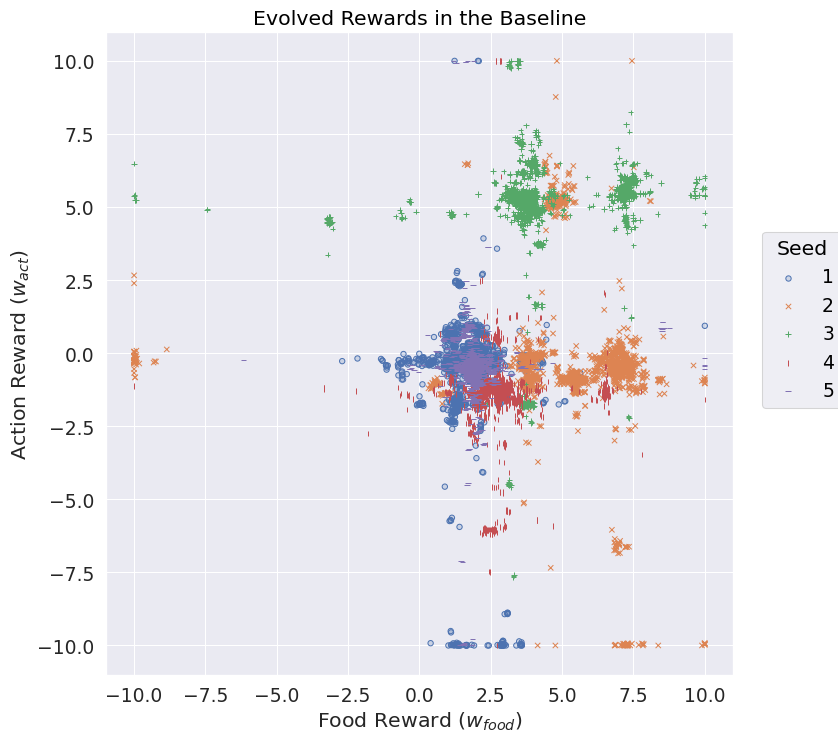
\includegraphics[width=8cm]{baseline-2d-sparse.png}
  \caption{
    Evolved rewards of agents born in the last $\num{1e6}$ steps in the baseline setting.
    The x-axis shows the weight for the food reward ($w_{\mathrm{food}}$), and the y-axis shows the weight for the action reward ($w_{\mathrm{act}}$).
    Different colors and marker shapes correspond to runs with different random seeds.
  }\label{figure:result-baseline}
\end{figure}

\section{Results}
In this section, we show our simulation results. We first show that biologically plausible reward functions evolve in our framework and then examine the effect of several environmental conditions, including metabolic balance, food density, and food relocation. Furthermore, we conduct experiments with poor or poisonous foods and examine their effect on evolved rewards.

As a baseline environment, we use the setting where food is always regenerated in the upper right area of the 2D environment, as the left figure in \Cref{figure:env} shows. All experiments start from $50$ agents with an energy level of $40.0$. Birth and hazard parameters in \Cref{table:hb} are tuned so that the population size is around $130\sim 150$ through evolution. Initial reward weights are sampled from a zero-mean Gaussian distribution with a standard deviation of $0.1$, so they should take values close to $0$. We conducted about ten million steps ($\num{1024e4}$) of the simulation, resulting in $300$ to $400$ generations, which takes $14\sim16$ hours on NVIDIA P100 GPU.

\Cref{figure:result-baseline} shows the reward weights of agents born in the last $1\%$ of steps ($\num{1e5}$ steps) with 5 random seeds in the baseline environment. Food rewards are almost positive in all 5 runs, and action rewards tend to be negative in the majority of runs. Thus, we can say that agents have acquired rewards that contribute to increasing their energy levels through evolution from scratch. However, there are some cases where action rewards are largely positive, which can lead to too much energy consumption and early death. Especially in the run with seed $3$, most of the agents have largely positive action rewards. This actually affects the population size badly. This run has the lowest average population size of $120.6$ in the last $\num{3e6}$ steps, while it is from $136$ to $149$ in other runs with negative action rewards. We suspect that this unfavorable reward for population growth can be chosen when there is no competition with other species and sufficient energy resources.

\begin{figure}[t]
  \begin{subfigure}[t]{8cm}
    \centering
    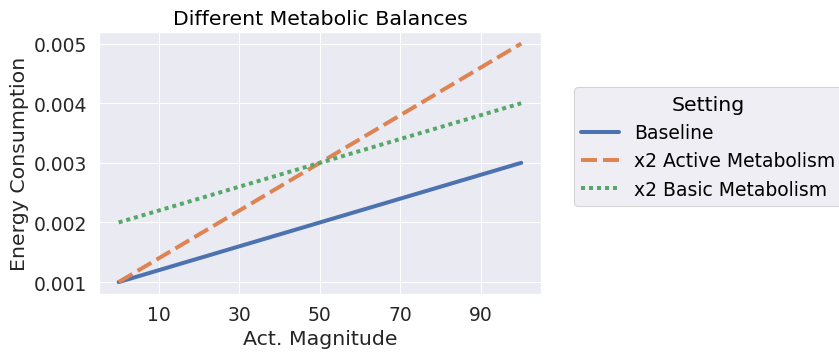
\includegraphics[width=8cm]{metabo-balance.png}
  \end{subfigure}
  \caption{
    Different metabolic balances we consider in experiments. The x-axis shows the action magnitude, and the y-axis shows the corresponding energy consumption.
  }\label{figure:metabo-balance}
\end{figure}

\begin{figure}[t]
  \centering
  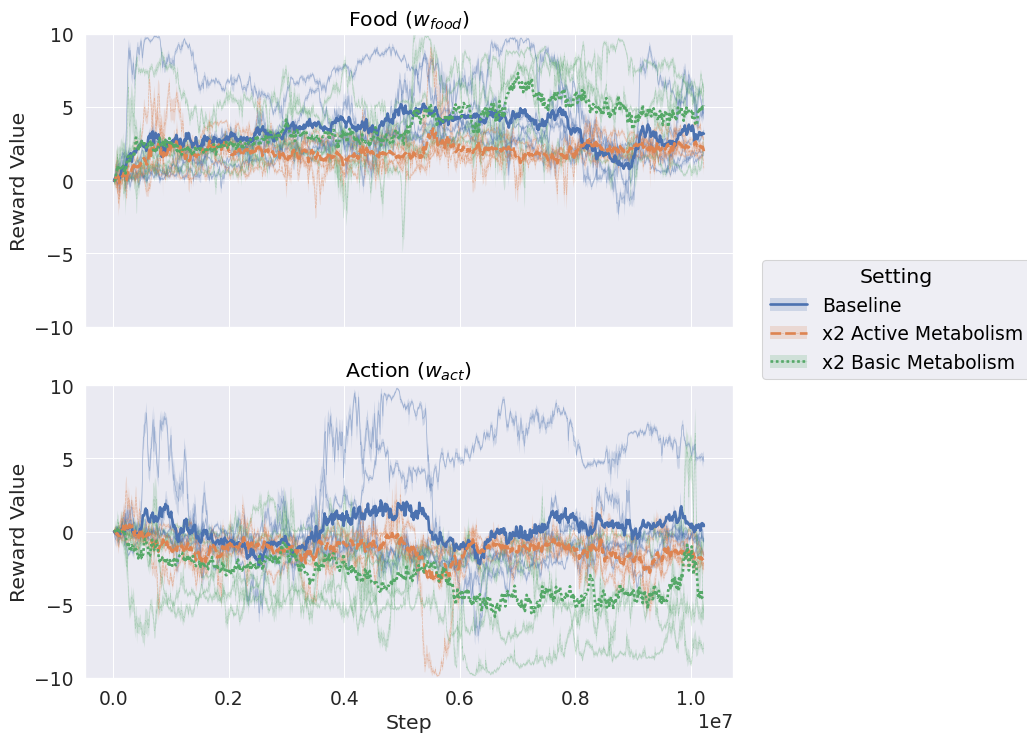
\includegraphics[width=8cm]{comp-metabo.png}
  \caption{
    Comparison of evolved rewards between different metabolic balances by different colors.
    The upper row shows the reward weight for food ($w_{\mathrm{food}}$), and the lower row shows the reward weight for action ($w_{\mathrm{act}}$).
    Each line shows the reward weight averaged over all agents alive at that time, while thin lines show the averages within one random seed.
  }\label{figure:result-metabolism}
\end{figure}

\paragraph{Effect of Metabolic Balance}
To investigate the effect of metabolic balance on rewards, we run simulations with two different metabolic balances. One has double active metabolism ($e_{\mathrm{act}} = \num{4e-5}$, \texttt{x2 Active Metabolism}), and the other has double the basic metabolism ($e_{\mathrm{basic}} = 0.002$, \texttt{x2 Basic Metabolism}). We show the difference between these two settings in \Cref{figure:metabo-balance}. While \texttt{x2 Basic Metabolism} consumes more energy for smaller action magnitude, \texttt{x2 Active Metabolism} consumes more when the action magnitude is larger than $50$.


\begin{figure}[t]
  \begin{subfigure}[t]{7cm}
    \centering
    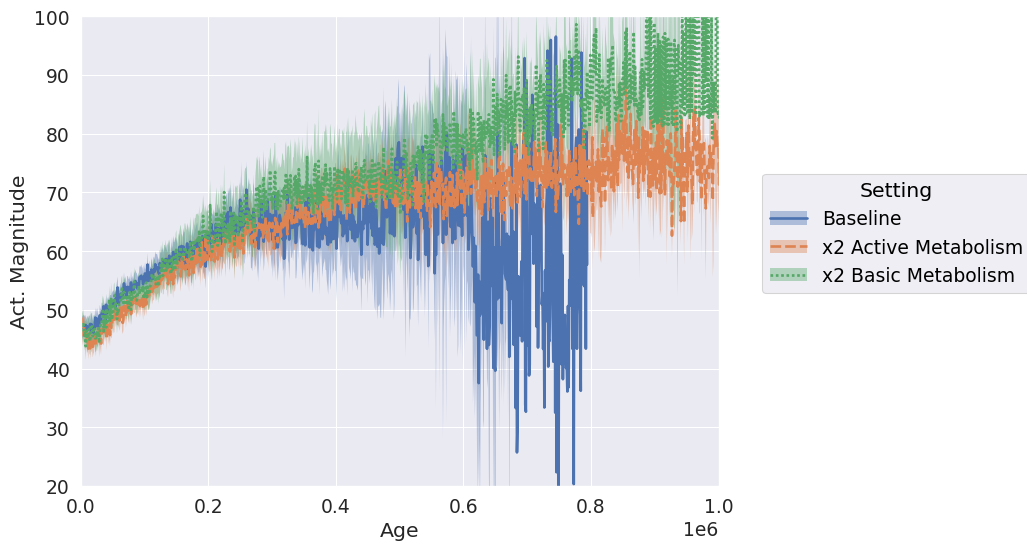
\includegraphics[width=7cm]{age-act.png}
  \end{subfigure}
  \caption{
    Change of the average action magnitude over aging only for agents who lived longer than $\num{1e5}$ steps.
    Specifically, agents with more than $60$ average action norm and more than $10$ children are selected for visualization.
  }\label{figure:actnorm-age}
\end{figure}

\Cref{figure:result-metabolism} compares the results between the baseline, \texttt{x2 Active Metabolism}, and \texttt{x2 Basic Metabolism}. The upper row shows the reward weight for food ($w_{\mathrm{food}}$), and the lower row shows the reward weight for action ($w_{\mathrm{act}}$). Each line shows the reward weight averaged over all agents alive at that time, while thin lines show the average within one random seed, resulting in five lines per different setting. In the two settings other than the baseline, we don't see any case where action rewards are significantly positive because of more severe energy consumption. Interestingly, we observe some cases with large food rewards and small action rewards only when the basic metabolism is doubled. To investigate the reason, we plot the learning curve for the average of action magnitude ($|a_{t}^{i}|$) over age for agents that lived longer than $1e5$ steps. We can observe that the average action magnitude is lower than $50$ for agents in their early ages, and doubling basic metabolism is harsher for younger agents. Surprisingly, in the double basic metabolism setting, agents tend to output larger actions, especially in their later lives, while they have more negative action rewards. This result shows that the strongness of survival pressure at early ages affects more on the shape of the reward function. It is also interesting that none of the agents in the baseline lived longer than $\num{5e8}$ steps, which implies that more harsh environmental conditions can lead to better rewards in terms of an individual's longevity.

\begin{figure}[t]
  \begin{subfigure}[t]{4cm}
    \centering
    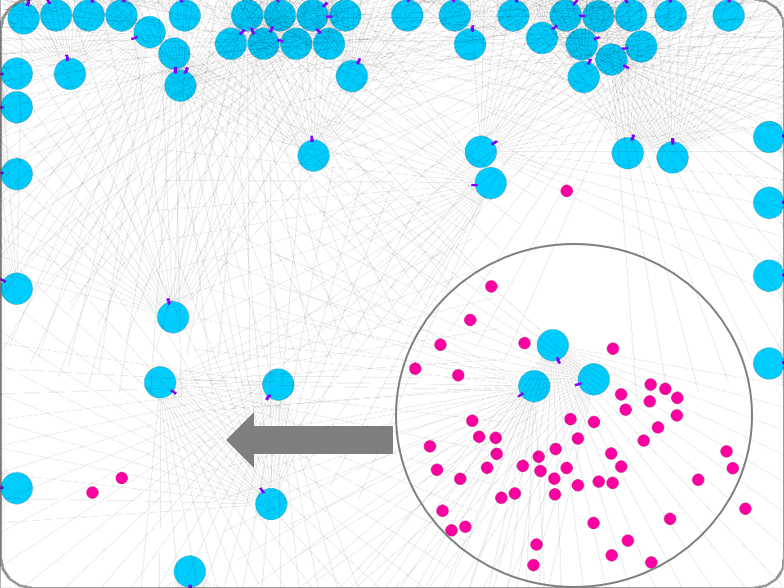
\includegraphics[width=4cm]{moving-annot-min.png}
  \end{subfigure}
  \begin{subfigure}[t]{4cm}
    \centering
    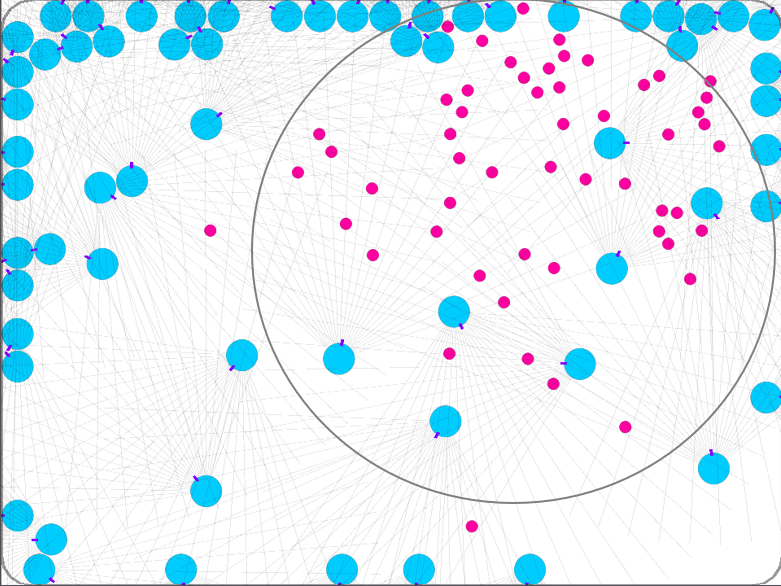
\includegraphics[width=4cm]{lv-annot-min.png}
  \end{subfigure}
  \caption{
    \textbf{Left:} Environment with food relocation.
    \textbf{Right:} Environment with spread foods.
  }\label{figure:foodloc}
\end{figure}

\begin{figure}[ht]
  \centering
  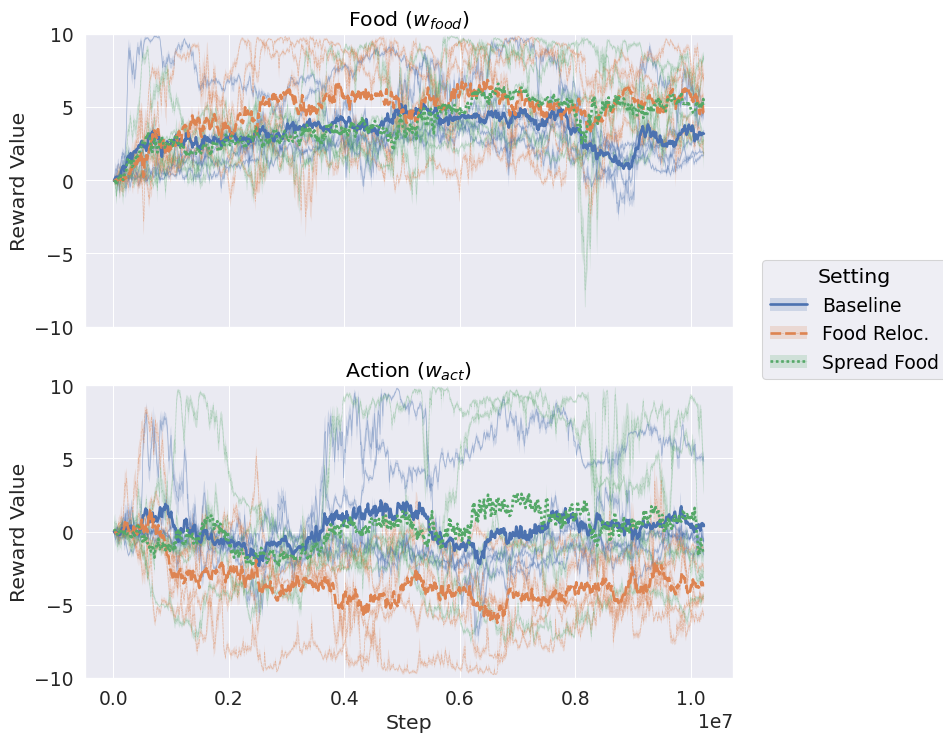
\includegraphics[width=8cm]{comp-loc.png}
  \caption{
    Comparison of evolved rewards between different food settings by different colors.
    The upper row shows the reward weight for food ($w_{\mathrm{food}}$), and the lower row shows the reward weight for action ($w_{\mathrm{act}}$).
    Each line shows the reward weight averaged over all agents alive at that time, while thin lines show the averages within one random seed.
  }\label{figure:result-foodloc}
\end{figure}

\begin{figure}[!htb]
  \centering
  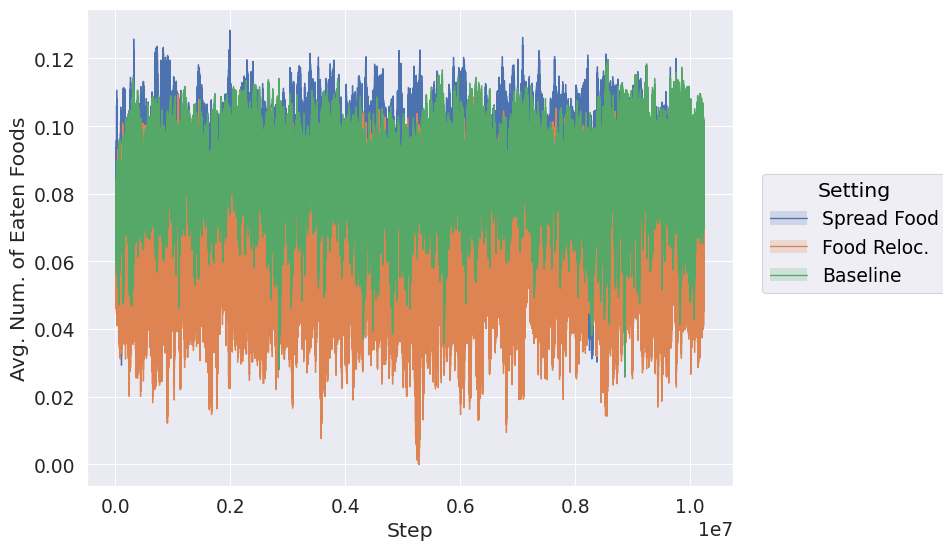
\includegraphics[width=8cm]{moving-nfoods.png}
  \caption{
    Comparison of the average number of foods that agents ate between different food locations.
    Rolling means over 10000 steps are taken for clear visualization.
  }\label{figure:result-nfood}
\end{figure}

\paragraph{Effect of Food Density and Relocation}
In the baseline setting, the center of the food location is a fixed location with a small variance, which can make the agents less active. The penalty for motor action can be smaller when agents need to hunt foods more actively. To confirm this hypothesis, we compare the evolved rewards in the baseline environment with ones in the environment where the food relocation happens clockwise (\texttt{Food Reloc.}) and the environment with more spread foods (\texttt{Spread Food}) shown in \Cref{figure:foodloc}. Note that in the food relocation setting, the center of food reproduction moves slightly clockwise after 100 foods are eaten.

We show the results in \Cref{figure:result-foodloc}. As our hypothesis suggests, action rewards are more likely to be positive in the spread food setting. However, contradicting our hypothesis, action rewards tend to be more negative in the food reloaction. To investigate the reason, we plot the rolling mean of the number of foods that agents ate in \Cref{figure:result-nfood}. We can see that getting food is more difficult in the \texttt{Food Reloc.} setting, which may lead to more negative action rewards.

\paragraph{Effect of Poor and Poisonous Foods}

\begin{figure}[t]
  \begin{subfigure}[t]{4cm}
    \centering
    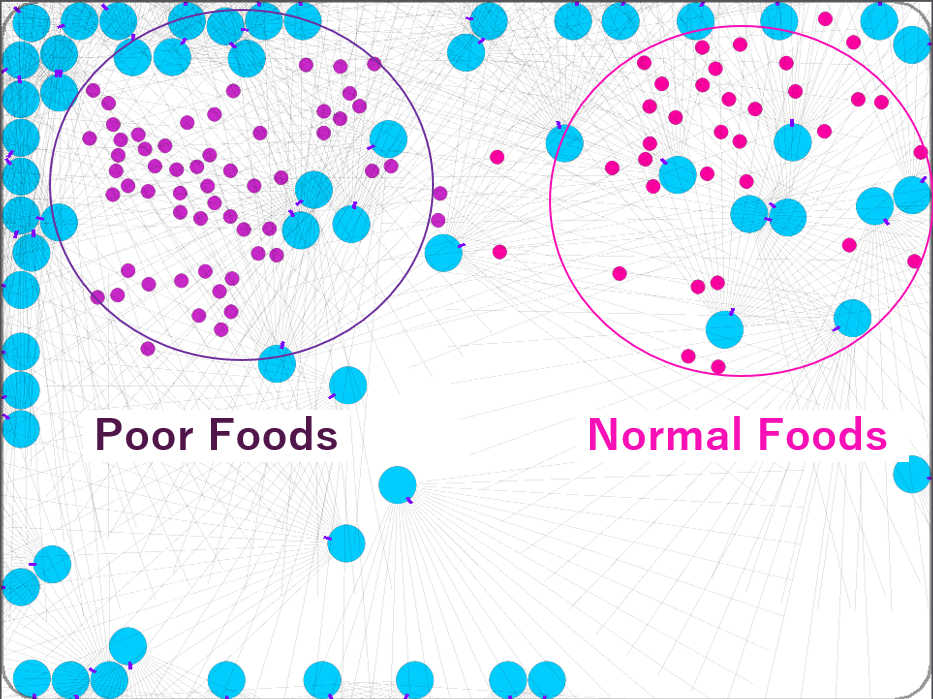
\includegraphics[width=4cm]{poor-annot-min.png}
  \end{subfigure}
  \begin{subfigure}[t]{4cm}
    \centering
    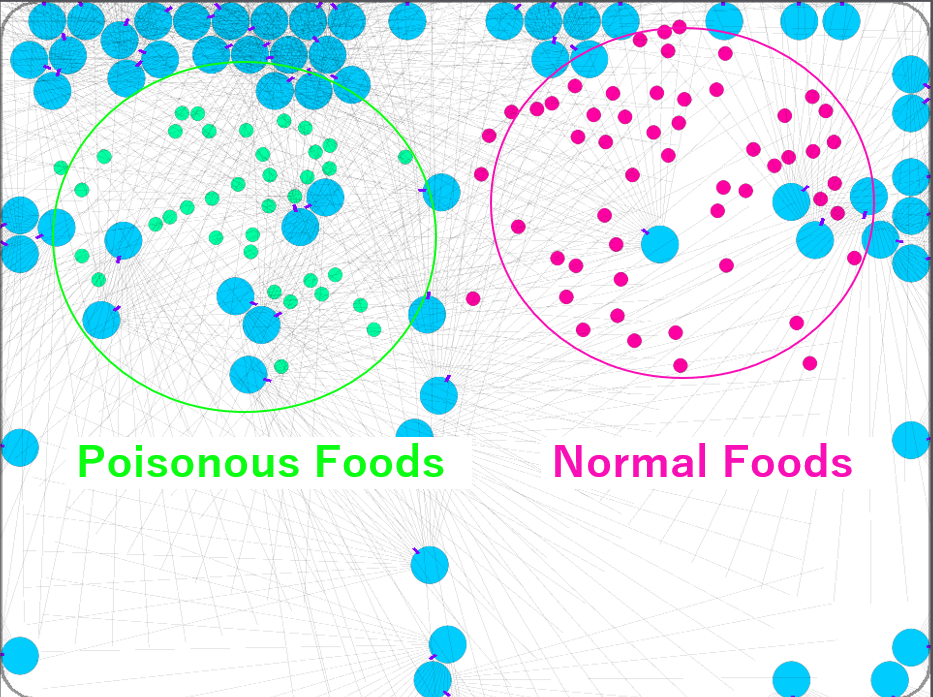
\includegraphics[width=4cm]{poison-annot-min.png}
  \end{subfigure}
  \caption{
    \textbf{Left:} Environment with poor foods.
    \textbf{Right:} Environment with poisonous foods.
  }\label{figure:pp}
\end{figure}

\begin{table}[t]
  \begin{subtable}[h]{0.45\columnwidth}
    \centering
    \begin{tabular}{cc}
      \toprule
      Parameter & Value \\
      \midrule
      $n_{\textrm{max}}^{\textrm{normal}}$ & 40\\
      $g^{\textrm{normal}}$ & 0.01 \\
      $n_{\textrm{max}}^{\textrm{poor}}$ & 60 \\
      $g^{\textrm{poor}}$ & 0.02 \\
      \bottomrule
    \end{tabular}
  \end{subtable}
  \begin{subtable}[h]{0.45\columnwidth}
    \centering
    \begin{tabular}{cc}
      \toprule
      Parameter & Value \\
      \midrule
      $n_{\textrm{max}}^{\textrm{normal}}$ & 60\\
      $g^{\textrm{normal}}$ & 0.01 \\
      $n_{\textrm{max}}^{\textrm{poison}}$ & 40 \\
      $g^{\textrm{poison}}$ & 0.01 \\
      \bottomrule
    \end{tabular}
  \end{subtable}
  \caption{
    Food regeneration parameters with poor foods (left) or poisonous foods (right).
    $n_{\textrm{max}}^{\textrm{poor}}$ and $n_{\textrm{max}}^{\textrm{poison}}$ are the maximum number of poor or poisonous foods, while $g^{\textrm{poor}}$ and $g^{\textrm{poison}}$ are growth rate of poor or poisonous foods.
  }\label{table:pp}
\end{table}

In the experiments so far, there is only one kind of food with $e_{\mathrm{food}} = 1.0$ in the environment. However, one role of our reward system is to distinguish between different external stimuli. For example, our food reward system helps us eat nutritious food, avoiding poisonous foods. Therefore, we conduct simulations with poor and poisonous foods, of which the energy gains are $e_{\mathrm{poor}} = 0.2$ and $e_{\mathrm{poison}} = -0.4$. In \Cref{figure:pp}, we show environments with poor and poisonous rewards. In those environments, we fix the center of poor or poisonous food location at the upper left. The number of maximum foods is smaller in the environment with poor foods, and there are more normal foods in the environment with poisonous foods as shown in \Cref{table:pp}, so the overall energy supply should be roughly the same.

\begin{figure}[t]
  \centering
  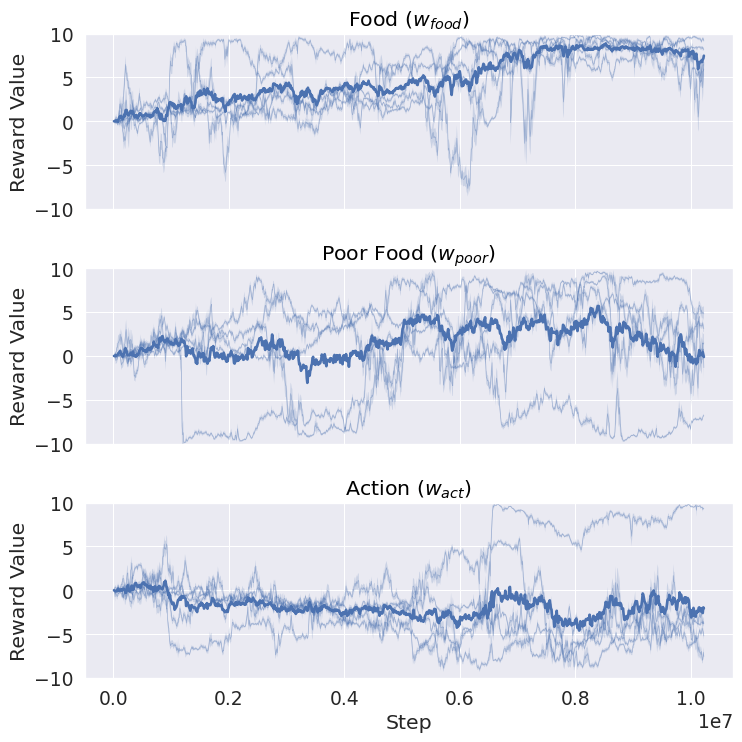
\includegraphics[width=8cm]{dyn-poor.png}
  \caption{
    Evolved rewards with poor foods.
    From top to bottom, each row shows the reward weight for food ($w_{\mathrm{food}}$), the reward weight for poor food ($w_{\mathrm{poor}}$), and the reward weight for action ($w_{\mathrm{act}}$).
    Each line shows the reward weight averaged over all agents alive at that time, while thin lines show the averages within one random seed.
  }\label{figure:result-poor}
\end{figure}

\begin{figure}[t]
  \centering
  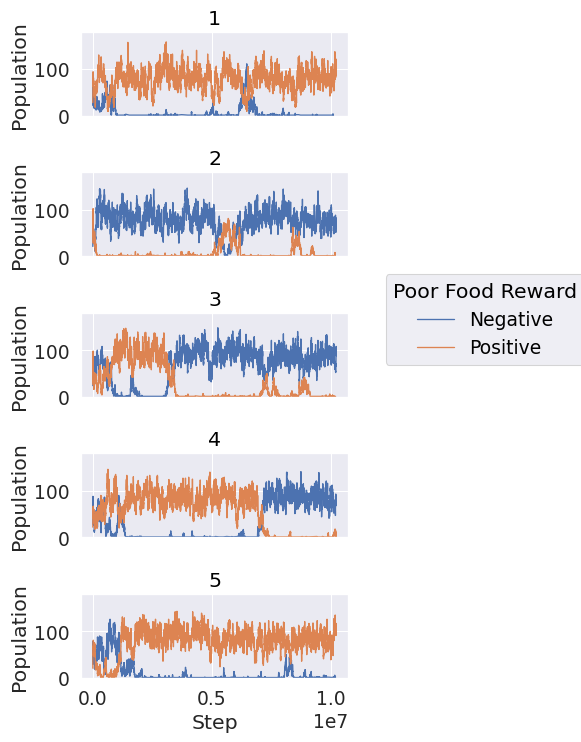
\includegraphics[width=6cm]{poor-pop.png}
  \caption{
    The population of agents with positive or negative rewards for poor foods in each seed.
    Blue lines show the population of agents with positive reward for poor foods, while orange lines shows the population of agents with negative ones.
  }\label{figure:pop-poor}
\end{figure}

\Cref{figure:result-poor} shows the evolution of reward weights with poor foods. The thick line shows the reward weight averaged over all agents alive at that time, while thin lines show the average between each random seed. From top to bottom, each row shows the reward weight for food ($w_{\mathrm{food}}$), the reward weight for poor food ($w_{\mathrm{poor}}$), and the reward weight for action ($w_{\mathrm{act}}$). Same as previous experiments, we used $5$ different random seeds. We can see that the reward weight for nomal food ($w_{\mathrm{food}}$) is consistently positive, while the other two rewards have great diversity. Thus, we can say that rewards for actions and poor foods are not very important in this environment, even if they help conserve or acquire energy.

To see whether speciation in terms of different rewards for poor foods happening, we compare the population of groups with positive or negative poor food rewards in \Cref{figure:pop-poor}.
Interestingly, we rarely see that the groups with different poor food rewards co-exist, although it is benefitial to avoiding population densification. They sometimes co-exist, but eventually one group take over others. Thus, we can see that there is rather an advantage in forming groups with a single genetic population in this environment. This result suggests that speciation may need alternative factors, such as geographic isolation and sexual reproduction.

\begin{figure}[t]
  \centering
  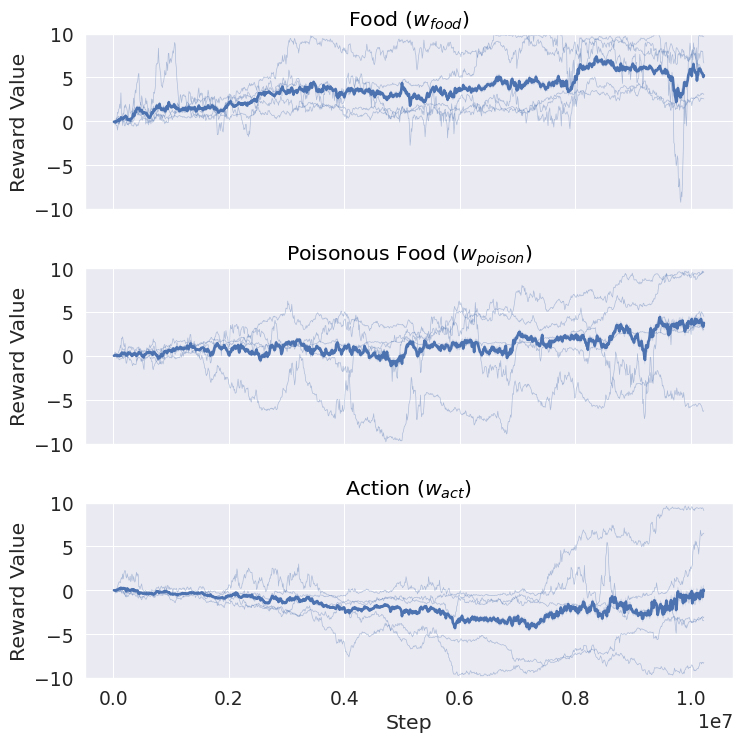
\includegraphics[width=8cm]{dyn-poison.png}
  \caption{
    Evolved rewards with poisonous foods.
    From top to bottom, each row shows the reward weight for food ($w_{\mathrm{food}}$), the reward weight for poisonous food ($w_{\mathrm{poison}}$), and the reward weight for action ($w_{\mathrm{act}}$).
    Each line shows the reward weight averaged over all agents alive at that time, while thin lines show the averages within one random seed.
  }\label{figure:result-poison}
\end{figure}

\begin{figure}[t]
  \centering
  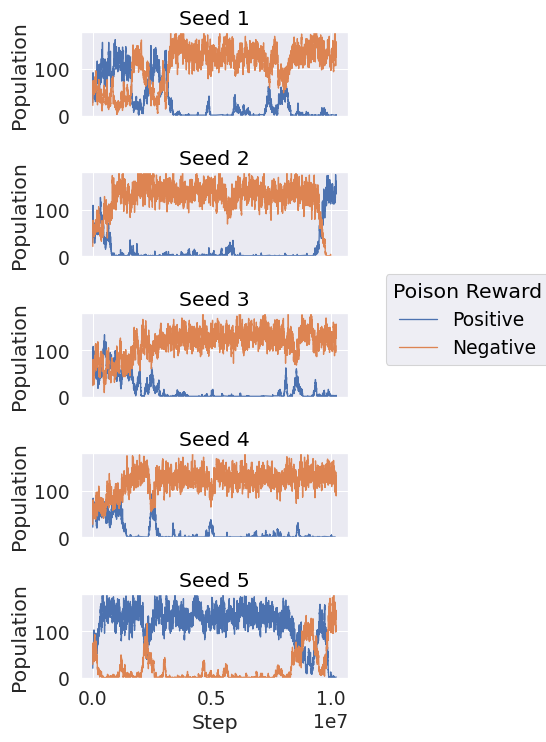
\includegraphics[width=6cm]{poison-pop.png}
  \caption{
    The population of agents with positive or negative rewards for poor foods.
    Blue lines show the population of agents with positive poison rewards, while orange lines shows the population of agents with negative ones.
  }\label{figure:pop-poison}
\end{figure}


\Cref{figure:result-poison} shows the evolution of reward weights with poisonous foods. Same as \Cref{figure:result-poor}, the thick line shows the reward weight averaged over all agents alive at that time, while thin lines show the average between each random seed. Again, we can see that the reward weight for nomal food ($w_{\mathrm{food}}$) is consistently positive. The other two reward are unstable and diverse, but we see that rewards for poison foods and actions are less often positive. We suspect that the existence of poisonous foods give stronger selection pressure to agents.

We compare the population of groups with positive or negative poison rewards in \Cref{figure:pop-poison}. We can see the same tendency as the case with poor foods. We rarely see the co-existance of agents with different poison rewards, and a single genetic population is preffered.

\section{Conclusion}
In this paper, we propose a distributed evolution framework with an energy-based birth and death model to study the evolution of reward function. Our GPU-based fast simulation enables to simulate millions of steps of evolution in a few hours. Our results show that biologically reasonable reward functions can evolve from randomly initialized ones. We also find that some environmental conditions, including metabolic balance, food density, and food relocation, can change the selection pressure and influence action rewards, while food rewards are consistently positive. Moreover, we examine the evolution of rewards for poor and poisonous rewards, finding that rewards for such less important foods can be unstable, although rewards for normal foods are consistenly positive. These results suggests that the evolution of reward function is lead by one nominal reward, in our case, the reward for normal food. The other components of rewards can be quite unstable even if they are benefitial for surival. One interesting future direction is to see the effect of competition between two species with, for example, in a predator-and-pray relationship.
